\documentclass{mwrep}

% Polskie znaki
\usepackage{polski}
\usepackage[utf8]{inputenc}
\usepackage[T1]{fontenc}
\usepackage{lmodern}
\usepackage{indentfirst}

% Strona tytułowa
\usepackage{pgfplots}
\usepackage{siunitx}
\usepackage{paracol}

% Pływające obrazki
\usepackage{float}
\usepackage{svg}
\usepackage{graphicx}

% table of contents refs
\usepackage{hyperref}
\usepackage{cleveref}
\usepackage{booktabs}
\usepackage{listings}
\usepackage{threeparttable}


\SendSettingsToPgf
\title{\bf System biurowych zakładów wzajemnych \vskip 0.1cm}
\author{Robert Wojtaś \and Jakub Sikora}
\date{\today}
\pgfplotsset{compat=1.15}	
\begin{document}

\makeatletter
\renewcommand{\maketitle}{\begin{titlepage}
		\begin{center}{
				\LARGE {\bf Politechnika Warszawska}}\\
			\vspace{0.4cm}
			{\LARGE {\bf Wydział Elektroniki i Technik Informacyjnych}}\\
			\vspace{5cm}
			{\bf \LARGE \mbox{Wprowadzenie do Baz Danych - Projekt} \vskip 0.1cm}
		\end{center}
		\vspace{0.1cm}

		\begin{center}
			{\bf \LARGE \@title}
		\end{center}

		\vspace{10cm}
		\begin{paracol}{2}
			\addtocontents{toc}{\protect\setcounter{tocdepth}{1}}
			\subsection*{Zdający:}
			\bf{ \Large{ \noindent\@author \par}}
			\addtocontents{toc}{\protect\setcounter{tocdepth}{2}}

			\switchcolumn \addtocontents{toc}{\protect\setcounter{tocdepth}{1}}
			\subsection*{Prowadzący:}
			\bf{\Large{\noindent \mbox{dr inż. Marcin Kowalczyk}}}
			\addtocontents{toc}{\protect\setcounter{tocdepth}{2}}

		\end{paracol}
		\vspace*{\stretch{6}}
		\begin{center}
			\bf{\large{Warszawa, \@date\vskip 0.1cm}}
		\end{center}
	\end{titlepage}
}
\makeatother
\maketitle

\tableofcontents
\listoftables
\listoffigures


\chapter{Zakres i cel projektu}

\section{Cel projektu}
Celem projektu jest poprawne zaprojektowanie relacyjnej bazy danych oraz jej
fizyczna implementacja przy użyciu systemu Oracle. W trakcie projektowania należy
odpowiednio podzielić fazy projektowania na poziom konceptualny oraz logiczny a także 
doprowadzić projekt bazy do trzeciej postaci normalnej.

\section{Założenia projektowe}
Realizowany projekt dotyczy biurowego systemu obstawiania meczów
na dużych turniejach sportowych. System ten zajmuje się zbieraniem 
zakładów od swoich użytkowników oraz prowadzeniem statystyk. 
Oferuje swoim użytkownikom możliwość zakładania się na wyniki spotkań
rozgrywanych w ramach uprzednio zdefiniowanych turniejów oraz podliczaniem 
wyników wedle ustalonego algorytmu punktowania.
\\ 
\\
\indent W tym celu, system prowadzi bazę danych która zbiera informacje o spotkaniach
oraz dostępnych turniejach. Każdy uczestnik gry próbuje przewidzieć dokładny wynik 
spotkania i w zależności od poprawności, otrzymuje $3$, $1$ albo $0$ punktów.
Trzy punkty gracz otrzymuje, gdy padnie dokładnie obstawiony przez niego wynik.
Gracz otrzymuje jeden punkt, gdy końcowy rezultat jest taki sam jak obstawiony z dokładnością
do zdobytych przez drużynę punktów. Przykładowo, gracz obstawił że meczu piłki
nożnej zakończy się rezultatem $3$:$1$ a mecz zakończył się wynikiem $4$:$2$. 
Gdy gracz nie trafi w rezultat, nie otrzymuje punktów.  
\\
\\
\indent W celu ułatwienia graczom podejmowanie decyzji, system oferuje szeroką gamę statystyk 
prowadzonych w ramach turniejów. Baza przechowuje informacje o nadchodzących spotkaniach 
pomiędzy dwoma drużynami, o zawodnikach występujących w tych drużynach, o sędziach 
przewidzianych do prowadzania danego spotkania a także o planowanym miejscu rozegrania spotkania.  
\\
\\
\indent Każdy użytkownik może grać niezależnie w kilku różnych turniejach i dodawać zakłady 
na dowolną ilość spotkań z takim zastrzeżeniem, że nie wolno dodać zakładu na 
rozpoczęte już spotkania. Dodatkowo, każdy turniej oferuje specjalne zakłady długoterminowe
dotyczące ostatecznego zwycięzcy i najbardziej wartościowego zawodnika turnieju. Zakłady 
te są warte odpowiednio więcej punktów. Po zakończeniu wszystkich spotkań z danego turnieju, wybierany 
jest zwycięzca na podstawie zdobytej liczby punktów. 


\chapter{Definicja systemu}

\section{Perspektywy użytkowników}
W ramach systemu zdefiniowaliśmy trzy typy potencjalnych użytkowników: \\
\begin{enumerate}
    \item Użytkownik - uczestnik gry, dodaje zakłady nierozpoczęte jeszcze spotkania w
    ramach turniejów na które się wcześniej zapisał\\ 

    \item Statystyk - moderator gry, dodaje informacje o drużynach, sędziach, stadionach i trenerach
    oraz na bieżąco uzupełnia wyniki spotkań i turniejów \\ 

    \item Administrator - główny moderator systemu, tworzy konta użytkownikom oraz przywraca dostępy \\
    
\end{enumerate}

\section{Zdefiniowane funkcjonalności}
Do zdefiniowania funkcjonalności posłużyliśmy się metodyką User Stories znanych z metodyki Agile. Wcieliśmy się 
w rolę każdego z użytkowników i opisaliśmy potrzebne funkcjonalności według znanego schematu:

\begin{center}
    \emph{Jako} osoba ..., \\ \emph{potrzebuję/chcę} takiej funkcjonalności ...,\\  \emph{ponieważ} pozwoli mi to ...  
\end{center}

Na podstawie tak opisanych funkcjonalności, w łatwy sposób mogliśmy zdefiniować potrzebne transakcje w systemie. Dodatkowo,
taki sposób opisu funkcjonalności już na etapie projektowania sprawdza ich przydatność.

\subsection{Użytkownik systemu}

\subsubsection{Zapis na turniej}
\emph{Jako użytkownik, potrzebuję mieć możliwość zapisania się na turniej, ponieważ wtedy będę mógł wziąć udział w grze.}

\subsubsection{Dodawanie zakładu na spotkanie}
\emph{Jako użytkownik, potrzebuję móc dodawać nowe zakłady na spotkania które jeszcze się nie rozpoczęły, ponieważ pozwoli mi to na zdobywanie punktów.}

\subsubsection{Edycja zakładu na spotkanie}
\emph{Jako użytkownik, potrzebuję móc edytować swoje zakłady na spotkania które jeszcze się nie rozpoczęły, ponieważ pozwoli mi to na zmianę zdania i poprawienie swojego zakładu.}

\subsubsection{Dodawanie zakładu długoterminowego}
\emph{Jako użytkownik, potrzebuję móc dodawać zakład długoterminowy na zwycięzce turnieju na który się zapisałem a który jeszcze się nie rozpoczął, ponieważ dzięki temu będę mógł zdobyć więcej punktów.}

\subsubsection{Edycja zakładu długoterminowego}
\emph{Jako użytkownik, potrzebuję móc edytować zakład długoterminowego na zwycięzce turnieju na który się zapisałem a który jeszcze się nie rozpoczął, ponieważ pozwoli mi to na zmianę zdania i poprawienie swojego zakładu.}

\subsubsection{Podgląd tabeli}
\emph{Jako użytkownik, potrzebuję móc sprawdzać który jestem w tabeli wyników, ponieważ potrzebuję informacji o ewentualnym zwycięstwie.}

\subsection{Statystyk}
\subsubsection{Dodawanie turniejów}
\emph{Jako statystyk, potrzebuję możliwości dodawania turniejów, ponieważ wtedy użytkownicy będą mogli się na nie zapisywać.}

\subsubsection{Dodawanie meczów}
\emph{Jako statystyk, potrzebuję możliwości dodawania meczów w ramach turniejów, ponieważ wtedy użytkownicy będą mogli się próbować obstawić ich wynik.}

\subsubsection{Dodawanie drużyn}
\emph{Jako statystyk, potrzebuję możliwości dodawania drużyn do systemu, ponieważ wtedy będę mógł je podpinać pod turnieje.}

\subsubsection{Podpinanie drużyn do turniejów}
\emph{Jako statystyk, potrzebuję możliwości dodawania drużyn jako uczestników turniejów, ponieważ wtedy będę mógł dodawać mecze do turniejów pomiędzy nimi.}

\subsubsection{Dodawanie stadionów}
\emph{Jako statystyk, potrzebuję możliwości dodawania stadionów do systemu, ponieważ wtedy będę mógł podpinać stadiony do meczów.}

\subsubsection{Podpinanie stadionów}
\emph{Jako statystyk, potrzebuję możliwości podpinania stadionów do meczów, ponieważ wtedy użytkownicy będą więcej wiedzieli o meczu co pozwoli im lepiej obstawić.}

\subsubsection{Dodawanie sędziów}
\emph{Jako statystyk, potrzebuję możliwości dodawania sędziów, ponieważ wtedy będę mógł podpinać sędziów głównych do spotkań.}

\subsubsection{Podpinanie sędziów}
\emph{Jako statystyk, potrzebuję możliwości podpinania sędziów do meczów, ponieważ wtedy użytkownicy będą więcej wiedzieli o meczu co pozwoli im lepiej obstawić.}

\subsubsection{Dodawanie wyników meczów}
\emph{Jako statystyk, potrzebuję możliwości dodawania wyników zakończonych już spotkań, ponieważ wtedy użytkownicy będą mogli zweryfikować swoje zakłady.}

\subsubsection{Dodawania zwycięzców turniejów}
\emph{Jako statystyk, potrzebuję możliwości dodawania zwycięzców turniejów, ponieważ wtedy użytkownicy będą mogli zweryfikować swoje zakłady długoterminowe.}

\subsubsection{Aktualizowanie składów drużyn}
\emph{Jako statystyk, potrzebuję możliwości aktualizowania składów drużyn, ponieważ wtedy statystyki będą aktualne.}


\subsection{Administrator}
\subsubsection{Dodawanie użytkowników}
\emph{Jako administrator, potrzebuję możliwości tworzenia kont dla użytkowników, ponieważ wtedy będą mogli wziąc udział w grze.}

\subsubsection{Zmiana hasła użytkownika}
\emph{Jako administrator, potrzebuję możliwości zmiany hasła użytkownika, ponieważ wtedy będę mógł przywrócić dostęp tym którzy zapomnieli hasła.}


\chapter{Model konceptualny}
Modelem konceptualnym nazywamy pewną reprezentację obiektów świata rzeczywistego 
w uniwersalnym modelu niezależnym od implementacji \cite{Wrembel1}. Poprawny model 
konceptualny jest dobrym punktem wyjścia, ponieważ pozwala na przemyślenie jakie
dane tak naprawdę chcemy przechowywać w projektowanej bazie oraz pozwala na usystematyzowanie
związków między danymi.

\section{Definicja zbiorów encji określonych w projekcie}
Wymagany zbiór encji najłatwiej uzyskać poprzez wyodrębnienie rzeczowników z opisu projektu.
Na podstawie analizy założeń projektowych założyliśmy następujący zbiór encji:

\begin{itemize}
	\item Użytkownik
	\item Mecz
	\item Zakład
	\item Wynik
	\item Zakład długoterminowy
	\item Turniej
	\item Drużyna
	\item Stadion
	\item Trener
	\item Sędzia
	\item Zawodnik
\end{itemize}
 
\vspace{1cm}
\section{Ustalenie związków i ich typów między encjami}

\begin{threeparttable}[H]
	\begin{tabular}{|p{0.15\linewidth}|p{0.15\linewidth}|p{0.05\linewidth}|p{0.17\linewidth}|p{0.17\linewidth}|p{0.1\linewidth}|}
	\hline
	\multicolumn{2}{|p{0.3\linewidth}|}{Relacje biorące udział} & Typ & \multicolumn{2}{p{0.3\linewidth}|}{Obowiązkowość} & Stopień         \\ \hline
	Użytkownik & Zakład & 1:n & Obowiązkowy & Opcjonalny & binarny  \\ \hline
	Użytkownik & ZakładD\tnote{1} & 1:n & Obowiązkowy & Opcjonalny & binarny  \\ \hline
	Użytkownik & Turniej & n:m & Opcjonalny & Opcjonalny & binarny  \\ \hline
	Mecz & Zakład & 1:n & Obowiązkowy & Opcjonalny & binarny  \\ \hline
	Turniej & ZakładD\tnote{1} & 1:n & Obowiązkowy & Opcjonalny & binarny  \\ \hline
	Turniej & Mecz & 1:n & Obowiązkowy & Opcjonalny & binarny  \\ \hline
	Sędzia & Mecz & 1:n & Obowiązkowy & Opcjonalny & binarny  \\ \hline
	Stadion & Mecz & 1:n & Obowiązkowy & Opcjonalny & binarny  \\ \hline
	Wynik & Mecz & 1:1 & Opcjonalny & Obowiązkowy & binarny  \\ \hline
	Drużyna & ZakładD\tnote{1} & 1:1 & Obowiązkowy & Obowiązkowy & binarny \\ \hline
	Drużyna & Mecz & 2:n & Obowiązkowy & Opcjonalny & binarny  \\ \hline
	Turniej & Drużyna & n:m & Opcjonalny & Opcjonalny & binarny \\ \hline 
	Turniej & Drużyna & 1:n & Opcjonalny & Opcjonalny & binarny \\ \hline 
	Zawodnik & Drużyna & n:m & Obowiązkowy & Opcjonalny & binarny  \\ \hline
	Trener & Drużyna & n:m & Opcjonalny & Obowiązkowy & binarny  \\ \hline
	\end{tabular}
	\begin{tablenotes}
		\item [1] skrót od ZakładDługoterminowy
	\end{tablenotes}	
	\caption{Typy wszystkich związków w schemacie}
\end{threeparttable}

\subsubsection{Użytkownik - Zakład}
Związek użytkownika z zakładem odwzorowuje następującą zależność. Użytkownik stawia zakład. Każdy zakład ma swojego jednego właściciela którym jest dany użytkownik, natomiast jeden użytkownik może stawiać od zera do wielu zakładów.

\subsubsection{Użytkownik - ZakładDługoterminowy}
Związek użytkownika z zakładem długoterminowym jest przedstawieniem w systemie zdarzenia postawienia przez użytkownika zakładu długoterminowego. Użytkownik tworzy zakład długoterminowy,w ogólności może ich tworzyć wiele (może też nie stworzyć żadnego). Każdy zakład długoterminowy ma obowiązkowo swojego jedynego właściciela.

\subsubsection{Użytkownik - Turniej}
Związek pomiędzy użytkownikiem a turniejem symbolizuje zapis użytkownika na turniej. Na jeden turniej może być zapisanych od zera do wielu użytkowników. Każdy użytkownik może zapisać się od zera do wielu turniejów.

\subsubsection{Mecz - Zakład} 
Kolejny związek jest reprezentacją fizycznego połączenia meczu i zakładu. Jeden zakład przewiduje wynik
tylko jednego meczu. Na jeden mecz może być postawionych kilka zakładów, w szczególności zero.

\subsubsection{Turniej - ZakładDługoterminowy}
Każdy zakład długoterminowy przewiduje wynik dokładnie jednego turnieju. Na jeden turniej może zostać
postawionych od zera do wielu zakładów długoterminowych.

\subsubsection{Turniej - Mecz}
W ramach jednego turnieju rozgrywane jest od zera (sytuacja raczej dziwna, jednak możliwa zanim statystyk doda do turnieju drużyny oraz spotkania) do wielu
spotkań. Jeden mecz jest rozgrywany w ramach jednego turnieju, przy czym zgodnie z założeniem wykluczamy możliwość
obstawiania spotkań towarzyskich czyli takich które nie są rozgrywane w ramach żadnego turnieju.

\subsubsection{Sędzia - Mecz}
Reprezentuje sędziowanie meczu przez sędziego. Jeden sędzia może sędziować wiele spotkań (oczywiście nie równocześnie), natomiast 
jedno spotkanie ma tylko jednego sędziego głównego.

\subsubsection{Stadion - Mecz}
Podobnie jak w poprzednim związku, jeden mecz jest rozgrywany na jednym stadionie. Jeden stadion może być gospodarzem
wielu spotkań.

\subsubsection{Wynik - Mecz}
Każdy mecz kończy się jakimś wynikiem. Zdecydowaliśmy się na rozwiązanie w którym wynik meczu jest przechowywany w osobnej encji.
Jest to związek 1:1, jeden wynik obowiązkowo odpowiada jednemu spotkaniu. Warto zwrócić uwagę na opcjonalność związku ze strony encji meczu.
Mecz który się jeszcze nie zakończył, nie może posiadać wyniku (system nie przewiduje obstawiania ustawionych spotkań).

\subsubsection{Drużyna - Zakład Długoterminowy}
Reprezentuje przewidywany wynik zakładu długoterminowego. Jeden zakład długoterminowy przewiduje jednego zwycięzce danego turnieju. 
Dana drużyna może wielokrotnie zostać wybrana przez użytkownika jako potencjalny zwycięzca, choć wcale nie musi być wybrana kiedykolwiek.

\subsubsection{Drużyna - Mecz}
Związek reprezentuje uczestnictwo drużyn w meczu. Każdy mecz musi mieć swoich uczestników. Zgodnie z założeniem, system pozwala na 
obstawianie spotkań pomiędzy dwoma drużynami, nie będą obsługiwane dyscyplinu typu skoki narciarskie gdzie liczba uczestników jest różna od dwóch.
Jedna drużyna może grać wiele spotkań, w szczególności żadnego.


\subsubsection{Turniej- Drużyna }
W ramach jednego turnieju, gra w nim tylko określony zbiór drużyn. Zgodnie z założeniem, drużyny mogą być dynamicznie dodawane 
do turnieju dlatego też zakładamy że turniej może mieć zero uczestniczących drużyn. Z drugiej strony, jedna drużyna może brać udział 
w wielu turniejach czy chociażby w różnych edycjach tych samych rozgrywek.


\subsubsection{Turniej - Drużyna \emph{ponownie...}}
Turnieje i drużyny łączy jeszcze jeden związek, który zdecydowaliśmy się specjalnie wyróżnić. Drugi związek pomiędzy turniejem a drużyną, reprezentuje zwycięzcę turnieju. W przypadku zwycięzców turniejów, 
zdecydowaliśmy się na przedstawienie tego nie za pomocą kolejnej encji (tak jak w przypadku encji \emph{Wynik}), tylko 
przy pomocy związku. Jeden turniej ma jednego zwycięzce, który zostaje poznany po jego zakończeniu. Jedna drużyna może wygrywać kilka turniejów,
w szczególności nie musi wygrać jakiegokolwiek.


\subsubsection{Zawodnik - Drużyna}
Jedna drużyna w danym momencie może mieć zakontraktowanych wielu zawodników oraz dodatkowo mieć historię zakończonych kontraktów z 
jeszcze większą ilością sportowców. Z drugiej strony, jeden zawodnik w swojej karierze może być związany
kontraktem z wieloma drużynami. 


\subsubsection{Trener - Drużyna}
Podobnie jak w przypadku poprzedniego punktu, związek \emph{Trener - Drużyna} reprezentuje kontrakty trenerów z drużynami.
Jedna drużyna ma (zazwyczaj) jednego głównego trenera, jednak ma przeszłość z innymi szkoleniowcami. Z drugiej strony, jeden szkoleniowiec
może w swoim życiu być związany z kilkoma (rekordziści nawet z kilkunastoma) drużynami. 

\newpage

\section{Określenie atrybutów i ich dziedzin}
\vspace{1.5cm}
\subsubsection{Użytkownik}
\begin{table}[H]
	\begin{tabular}{|p{0.25\linewidth}|p{0.2\linewidth}|p{0.2\linewidth}|p{0.25\linewidth}|}
	\hline
	Nazwa atrybutu & Typ i dziedzina & Obowiązkowy? & Opis                                                           \\ \hline
	UżytkownikId   & liczbowy                            & TAK                              & Numer identyfikujący użytkownika                                                   \\ \hline
	Login          & napisowy                            & TAK                              & Login do systemu oraz nazwa pod którą użytkownik będzie widoczny w systemie         \\ \hline
	Hasło          & napisowy                            & TAK                              & Hash hasła, którym użytkownik będzie logował się do systemu                        \\ \hline
	Salt           & napisowy                            & TAK                              & Ciąg znaków zaburzający hasło, celem utrudnienia jego złamania                     \\ \hline
	Imię           & napisowy                            & TAK                              & Imię użytkownika, wymagane do identyfikacji i ewentualnego przekazania nagrody     \\ \hline
	Nazwisko       & napisowy                            & TAK                              & Nazwisko użytkownika, wymagane do identyfikacji i ewentualnego przekazania nagrody \\ \hline
	\end{tabular}
	\caption{Atrybuty encji Użytkownik}
\end{table}

\subsubsection{Mecz}
\begin{table}[H]
	\begin{tabular}{|p{0.25\linewidth}|p{0.2\linewidth}|p{0.2\linewidth}|p{0.25\linewidth}|}
	\hline
	Nazwa atrybutu & Typ i dziedzina & Obowiązkowy? & Opis                                                           \\ \hline
	MeczId   & liczbowy                            & TAK                              & Numer identyfikujący mecz                                                  \\ \hline
	DataRozpoczęcia          & datowy                            & TAK                              & Dzień i godzina rozpoczęcia meczu, do tego momentu można dodawać zakłady.       \\ \hline
	\end{tabular}
	\caption{Atrybuty encji Mecz}
\end{table}

\newpage

\subsubsection{Zakład}
\begin{table}[H]
	\begin{tabular}{|p{0.25\linewidth}|p{0.2\linewidth}|p{0.2\linewidth}|p{0.25\linewidth}|}
	\hline
	Nazwa atrybutu & Typ i dziedzina & Obowiązkowy? & Opis                                                           \\ \hline
	ZakładId   & liczbowy                            & TAK                              & Numer identyfikujący zakładu                                                   \\ \hline
	WynikGospodarzy         & liczbowy                           & TAK                              & Przewidywany wynik zdobyty przez drużynę gospodarzy         \\ \hline
	WynikGości          & liczbowy                            & TAK                              & Przewidywany wynik zdobyty przez drużynę gości                        \\ \hline
	DataZawarcia           & datowy                            & TAK                              & Data i godzina dodania/ostatniej edycji zakładu                 \\ \hline
	\end{tabular}
	\caption{Atrybuty encji Zakład}
\end{table}

\vspace{1cm}

\subsubsection{Wynik}
\begin{table}[H]
	\begin{tabular}{|p{0.25\linewidth}|p{0.2\linewidth}|p{0.2\linewidth}|p{0.25\linewidth}|}
	\hline
	Nazwa atrybutu & Typ i dziedzina & Obowiązkowy? & Opis                                                           \\ \hline
	WynikId   & liczbowy                            & TAK                              & Numer identyfikujący wynik                                                   \\ \hline
	WynikGospodarzy         & liczbowy                            & TAK                              & Faktyczny wynik zdobyty przez drużynę gospodarzy         \\ \hline
	WynikGości          & liczbowy                            & TAK                              & Faktyczny wynik zdobyty przez drużynę gości                        \\ \hline
	DataDodania           & datowy                            & TAK                              & Data i godzina dodania wyniku, potrzebna przy ewentualnej weryfikacji    \\ \hline
	\end{tabular}
	\caption{Atrybuty encji Wynik}
\end{table}

\vspace{1cm}

\subsubsection{Zakład Długoterminowy}
\begin{table}[H]
	\begin{tabular}{|p{0.25\linewidth}|p{0.2\linewidth}|p{0.2\linewidth}|p{0.25\linewidth}|}
	\hline
	Nazwa atrybutu & Typ i dziedzina & Obowiązkowy? & Opis                                                           \\ \hline
	ZakładDługotermi- nowyId   & liczbowy                            & TAK                              & Numer identyfikujący zakład długoterminowy                                                  \\ \hline
	DataZawarcia          & datowy                            & TAK                              & Data i godzina dodania/ostatniej edycji zakładu.       \\ \hline
	\end{tabular}
	\caption{Atrybuty encji Zakład Długoterminowy}
\end{table}

\newpage

\subsubsection{Turniej}
\begin{table}[H]
	\begin{tabular}{|p{0.25\linewidth}|p{0.2\linewidth}|p{0.2\linewidth}|p{0.25\linewidth}|}
	\hline
	Nazwa atrybutu & Typ i dziedzina & Obowiązkowy? & Opis                                                           \\ \hline
	TurniejId   & liczbowy                            & TAK                              & Numer identyfikujący turniej  \\ \hline
	Nazwa   & napisowy                            & TAK                              & Pełna nazwa turnieju  \\ \hline
	DataRozpoczęcia          & datowy                            & TAK                              & Data i godzina rozpoczęcia turnieju, tj. pierwszego spotkania w tym turnieju.       \\ \hline
	\end{tabular}
	\caption{Atrybuty encji Turniej}
\end{table}

\vspace{1cm}

\subsubsection{Drużyna}
\begin{table}[H]
	\begin{tabular}{|p{0.25\linewidth}|p{0.2\linewidth}|p{0.2\linewidth}|p{0.25\linewidth}|}
	\hline
	Nazwa atrybutu & Typ i dziedzina & Obowiązkowy? & Opis                                                           \\ \hline
	DrużynaId   & liczbowy                            & TAK                              & Numer identyfikujący drużynę                                                   \\ \hline
	Nazwa         & napisowy                           & TAK                              & Pełna nazwa drużyny         \\ \hline
	Miasto          & napisowy                            & TAK                              & Miasto z którego pochodzi drużyna                        \\ \hline
	Narodowość           & napisowy                            & TAK                              & Kraj z którego pochodzi drużyna                 \\ \hline
	\end{tabular}
	\caption{Atrybuty encji Drużyna}
\end{table}

\vspace{1cm}

\subsubsection{Stadion}
\begin{table}[H]
	\begin{tabular}{|p{0.25\linewidth}|p{0.2\linewidth}|p{0.2\linewidth}|p{0.25\linewidth}|}
	\hline
	Nazwa atrybutu & Typ i dziedzina & Obowiązkowy? & Opis                                                           \\ \hline
	StadionId   & liczbowy                            & TAK                              & Numer identyfikujący stadion                                                   \\ \hline
	Nazwa         & napisowy                           & TAK                              & Pełna nazwa areny         \\ \hline
	Pojemność 	   & liczbowy							& TAK								& Pojemność widowni \\  \hline
	Miasto          & napisowy                            & TAK                              & Miasto w którym znajduje się stadion                       \\ \hline
	Narodowość           & napisowy                            & TAK                              & Nazwa ulicy przy której znajduje się stadion   \\ \hline
	\end{tabular}
	\caption{Atrybuty encji Stadion}
\end{table}

\newpage

\subsubsection{Trener}
\begin{table}[H]
	\begin{tabular}{|p{0.25\linewidth}|p{0.2\linewidth}|p{0.2\linewidth}|p{0.25\linewidth}|}
	\hline
	Nazwa atrybutu & Typ i dziedzina & Obowiązkowy? & Opis                                                           \\ \hline
	TrenerId   & liczbowy                            & TAK                              & Numer identyfikujący trenera                                                   \\ \hline
	Imię         & napisowy                           & TAK                              & Imię/imiona trenera        \\ \hline
	Nazwisko	   & liczbowy							& TAK								& Nazwisko trenera \\  \hline
	DataUrodzenia          & datowy                           & TAK                              & Data urodzenia trenera              \\ \hline
	Narodowość           & napisowy                            & TAK                              & Kraj pochodzenia   \\ \hline
	\end{tabular}
	\caption{Atrybuty encji Trener}
\end{table}

\vspace{1cm}

\subsubsection{Sędzia}
\begin{table}[H]
	\begin{tabular}{|p{0.25\linewidth}|p{0.2\linewidth}|p{0.2\linewidth}|p{0.25\linewidth}|}
	\hline
	Nazwa atrybutu & Typ i dziedzina & Obowiązkowy? & Opis                                                           \\ \hline
	SędziaId   & liczbowy                            & TAK                              & Numer identyfikujący sędziego                                                   \\ \hline
	Imię         & napisowy                           & TAK                              & Imię/imiona sędziego        \\ \hline
	Nazwisko	   & liczbowy							& TAK								& Nazwisko sędziego \\  \hline
	DataUrodzenia          & datowy                           & TAK                              & Data urodzenia sędziego              \\ \hline
	Narodowość           & napisowy                            & TAK                              & Kraj pochodzenia   \\ \hline
	\end{tabular}
	\caption{Atrybuty encji Sędzia}
\end{table}

\subsubsection{Zawodnik}
\begin{table}[H]
	\begin{tabular}{|p{0.25\linewidth}|p{0.2\linewidth}|p{0.2\linewidth}|p{0.25\linewidth}|}
	\hline
	Nazwa atrybutu & Typ i dziedzina & Obowiązkowy? & Opis                                                           \\ \hline
	SędziaId   & liczbowy                            & TAK                              & Numer identyfikujący sędziego                                                   \\ \hline
	Imię         & napisowy                           & TAK                              & Imię/imiona sędziego        \\ \hline
	Nazwisko	   & liczbowy							& TAK								& Nazwisko sędziego \\  \hline
	DataUrodzenia          & datowy                           & TAK                              & Data urodzenia sędziego              \\ \hline
	Narodowość           & napisowy                            & TAK                              & Kraj pochodzenia   \\ \hline
	Numer           & liczbowy                            & TAK                              & Numer na koszulce   \\ \hline
	\end{tabular}
	\caption{Atrybuty encji Sędzia}
\end{table}

\section{Dodatkowe reguły integralnościowe}

Na poziomie konceptualnym, wszystkie atrybuty zostały oznaczone jako \texttt{NOT NULL}. Dodatkowo, atrybut \emph{Login} w encji
\emph{Użytkownik} musi być unikalny względem reszty danych w bazie, dlatego też został on opatrzony słowem \texttt{UNIQUE}.

Należy zapewnić aby w systemie nie doszło do sytuacji że zwycięzcą danego turnieju jest drużyna która nie jest jego uczestnikiem.
Zgodnie podjęliśmy decyzję projektową że to zabezpieczenie zostanie zrealizowane po stronie aplikacji a nie po stronie bazy danych.

\vspace{1cm}
\section{Klucze kandydujące i główne}

Dla każdej encji spróbowaliśmy znaleźć unikalny klucz. Wyniki naszych starań znajdują się w
tabeli poniżej.

\vspace{1cm}
\begin{threeparttable}[H]
	\begin{tabular}{|p{0.5\linewidth}|p{0.43\linewidth}|}
	\hline
	Relacja & Klucz kandydujący \\ \hline
	Użytkownik & Login \\ \hline
	Mecz &  \hfil--- \\ \hline
	Drużyna &  Nazwa \\ \hline
	Zawodnik &  Imię \& Nazwisko \\ \hline
	Stadion &  Adres \& Nazwa \\ \hline
	Zakład &  \hfil--- \\ \hline
	Wynik &  \hfil--- \\ \hline
	Turniej &  Nazwa \\ \hline
	Sędzia & Imię \& Nazwisko \\ \hline
	Trener & Imię \& Nazwisko \\ \hline
	ZakładDługoterminowy &  \hfil--- \\ \hline
	\end{tabular}	
	\caption{Proponowane klucze kandydujące}
\end{threeparttable}
\vspace{1cm}

W tabeli znajdują się niepoprawne klucze takie jak kombinację imienia i nazwiska, które należy z miejsca odrzucić, pomimo faktu że prawdopodobieństwo
istnienia dwóch zawodników o tym samym imieniu i nazwisku jest niezwykle niskie (niskie nie znaczy zerowe). 
Dodatkowo, doszliśmy do wniosku że nazwy turniejów z góry nie muszą być unikalne. To samo tyczy się nazw drużyn, które mogą
prowadzić różne sekcje o tej samej nazwie. Po kolei odrzucając kolejne klucze, zdecydowaliśmy że jedynym sensownym kluczem kandydującym
jest \emph{Login} w encji \emph{Użytkownik}, który musi być unikalny. \\
\\
Z tego też powodu podjęliśmy kolejną decyzją projektową jaką było wstawienie do każdej encji sztucznego klucza głównego 
w postaci liczbowego identyfikatora. 

\vspace{1cm}
\begin{threeparttable}[H]
	\begin{tabular}{|p{0.3\linewidth}|p{0.35\linewidth}|p{0.25\linewidth}|}
	\hline
	Relacja & Klucz główny & Klucz kandydujący \\ \hline
	Użytkownik & UżytkownikId & Login \\ \hline
	Mecz & MeczId & \hfil--- \\ \hline
	Drużyna & DrużynaId & \hfil--- \\ \hline
	Zawodnik & ZawodnikId & \hfil--- \\ \hline
	Stadion & StadionId & \hfil--- \\ \hline
	Zakład & ZakładId & \hfil--- \\ \hline
	Wynik & WynikId & \hfil--- \\ \hline
	Turniej & TurniejId & \hfil--- \\ \hline
	Sędzia & SędziaId & \hfil--- \\ \hline
	Trener & TrenerId & \hfil--- \\ \hline
	ZakładDługoterminowy & ZakładDługoterminowyId & \hfil--- \\ \hline
	\end{tabular}	
	\caption{Klucze główne i pozostałe kandydujące}
\end{threeparttable}
\vspace{1cm}

\newpage

\section{Problem pułapek szczelinowych i wachlarzowych – analiza i przykłady}
Przed przejściem do kolejnego etapu projektowania, należało rozważyć czy w naszym projekcie
nie ukryły się żadne pułapki szczelinowe oraz wachlarzowe. 


\subsection{Pułapki wachlarzowe}
Pułapką wachlarzową nazywamy sytuację w której nie ma jednoznacznego połączenia pomiędzy dwoma encjami które 
są w związku n:$1$ z tą samą encją. Najłatwiej ją zidentyfikować gdy z jednej encji wychodzi więcej niż jeden związek $1$:n.

\begin{figure}[H]
	\centering
	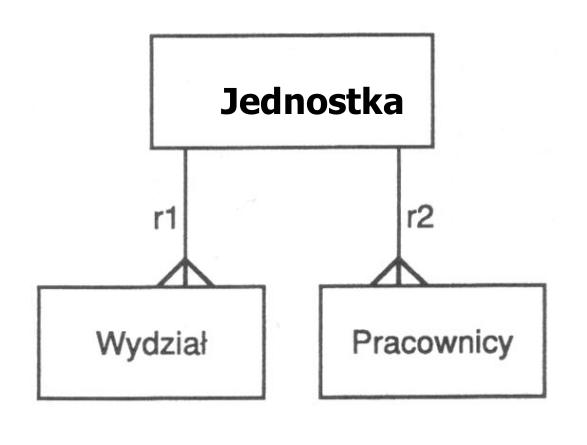
\includegraphics[scale=0.4]{./wachlarz.png}
	\caption{Przykład pułapki wachlarzowej przedstawionej na wykładzie\cite{Kowalczyk1}}
\end{figure}

Na przykładzie przedstawionym powyżej, nie jest możliwe jednoznaczne wywnioskowanie w którym wydziale pracuje dany pracownik, mimo iż znamy 
do której należy jednostki. \\
\\
\indent W początkowym projekcie systemu, do schematu wkradła nam się pułapka wachlarzowa pomiędzy encjami \emph{Użytkownik}, \emph{Turniej} oraz \emph{Zakład}.
Jej wynikiem był brak możliwości zapytania o wszystkie zakłady jednego użytkownika w ramach jednego turnieju. Pułapkę zlikwidowaliśmy
poprzez dodanie związku pomiędzy encjami \emph{Turniej} oraz \emph{Zakład}. Po takiej modyfikacji zakład przechowuje informację w ramach jakiego turnieju został on stworzony
co umożliwia zliczanie punktów.
\newpage
\subsection{Pułapki szczelinowe}
Pułapką szczelinową nazywamy sytuację w której nie ma jednoznacznego połączenia pomiędzy encjami, połączonych związkami $1$:n w następujący sposób.

\begin{figure}[H]
	\centering
	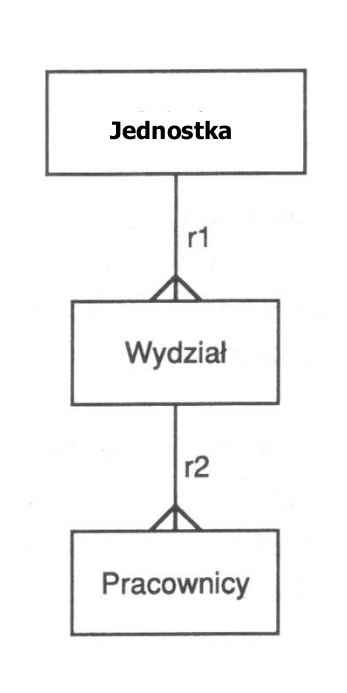
\includegraphics[scale=0.4]{./szczelina.png}
	\caption{Przykład pułapki szczelinowej przedstawionej na wykładzie\cite{Kowalczyk1}}
\end{figure}

Niepoprawnym jest założenie że zawsze znajdzie się połączenie po środku, brak połączenia nazywamy szczeliną. Rozwiązaniem 
tej sytuacji jest dodanie kolejnego związku między skrajnymi encjami. \\
\\
W przedstawionym projekcie, po wnikliwej analizie stwierdziliśmy brak sensownych pułapek szczelinowych, tj. istnieją 
takie połączenia spełniające wymagania pułapki szczelinowej ale z punktu biznesowego takie połączenia nie mają sensu, dlatego też 
zostają one świadomie pominięte.	

\section{Schemat ER na poziomie konceptualnym}
Schemat ER na poziome konceptualnym znajduje się w załączniku A dołączonym na końcu sprawozdania.

\chapter{Model logiczny}

\section{Charakterystyka modelu relacyjnego}
Model relacyjny został wprowadzony przez pracownika IBM, Edgara Franka Codda w 1970 roku\cite{Codd}. Model 
ten opisuje dane za pomocą tabel nazywanych relacjami, które przechowują atomowe dane. Na relacjach są dobrze
zdefiniowane operacje wyszukiwania, dodawania danych i ich edycji. Dodatkowo, w łatwy sposób 
definiowane są warunki spójności: zależności kluczowe i zawierania oraz ograniczenia na wartości danych poprzez
typy czy dopuszczalne zbiory wartości.\\
\\
\indent Daleko posunięta niezależność danych zezwala na modyfikacje wewnętrznej reprezentacji
danych, uporządkowania rekordów czystruktury plików bez wpływu na aplikacje
wykorzystujące dane.

\section{Usunięcie właściwości niekompatybilnych z modelem relacyjnym}
\subsection{Tablice bridge'ujące}
Najpoważniejszą niekompatybilnością logicznego modelu relacyjnego z modelem konceptualnym jest odwzorowanie związków
wiele do wielu. W modelu relacyjnym są one niedopuszczalne. Rozwiązaniem problemu jest wprowadzanie tablic bridge'ujących.
Pozwalają one na reprezentację związków wiele do wielu za pomocą kolumn odpowiadających kluczom głównym zbiorów encji biorących
udział w związku\cite{Kowalczyk1}.\\
\\
\indent W prezentowanym wcześniej modelu konceptualnym występowały cztery związki wiele do wielu: 
\\
\begin{itemize}
	\item \emph{Użytkownik} - \emph{Turniej}
	\item \emph{Drużyna} - \emph{Turniej}
	\item \emph{Drużyna} - \emph{Zawodnik}
	\item \emph{Drużyna} - \emph{Trener}
\end{itemize}
\vspace{0.5cm}
Dla każdego związku, stworzona została odpowiadająca jej tablica: \\
\\
\begin{threeparttable}[H]
	\begin{tabular}{|p{0.5\linewidth}|p{0.43\linewidth}|}
	\hline
	Związek n:m &  Bridge \\ \hline
	\emph{Użytkownik} - \emph{Turniej} & \emph{ZapisUżytkownika} \\ \hline
	\emph{Drużyna} - \emph{Turniej} &  \emph{ZapisDrużyny} \\ \hline
	\emph{Drużyna} - \emph{Zawodnik} &  \emph{KontraktZawodnika} \\ \hline
	\emph{Drużyna} - \emph{Trener} &  \emph{KontraktTrenerski} \\ \hline
	\end{tabular}	
	\caption{Zrealizowana zamiana związków wiele do wielu na tablice bridge'ujące}
\end{threeparttable}
\vspace{0.5cm}

Dodatkowo, do tablic \emph{KontraktZawodnika} i \emph{KontraktTrenerski} dodane zostały dodatkowe 
atrybuty \emph{DataZawarcia} i \emph{DataZakończenia}. Pozwala to na przechowywanie informacji o historii
(z zachowaniem chronologii) oraz informacji o tym który kontrakt jest aktualnie ważny (jest to ten bez 
daty zakończenia).

\subsection{Liczby mnogie}
W związku z inną konwencją nazewniczą, zmieniliśmy nazwy relacji tak aby ich nazwy były w liczbie mnogiej.\\
\\
\begin{threeparttable}[H]
	\begin{tabular}{|p{0.5\linewidth}|p{0.43\linewidth}|}
	\hline
	Stara nazwa & Nowa nazwa \\ \hline
	Użytkownik & Użytkownicy \\ \hline
	Mecz & Mecze \\ \hline
	Zakład & Zakłady \\ \hline
	Wynik & Wyniki \\ \hline
	ZakładDługoterminowy & ZakładyDługoterminowe \\ \hline
	Turniej & Turnieje \\ \hline
	Drużyna & Drużyny \\ \hline
	Stadion & Stadiony \\ \hline
	Trener & Trenerzy \\ \hline
	Sędzia & Sędziowie \\ \hline
	Zawodnik & Zawodnicy \\ \hline
	ZapisUżytkownika & ZapisyUżytkowników \\ \hline
	ZapisDrużyny & ZapisyDrużyn \\ \hline
	KontraktZawodnika & KontraktyZawodników \\ \hline
	KontraktTrenerski & KontraktyTrenerskie \\ \hline
	\end{tabular}	
	\caption{Zrealizowana zmiana nazw relacji}
\end{threeparttable}
\vspace{0.5cm}

\subsection{Typy danych}
W modelu konceptualnym, określiliśmy typy danych w sposób bardzo ogólny. Na tym etapie dokonamy ich 
specyfikacji, typowi liczbowemu przypisaliśmy typ \texttt{INTEGER}, typowi napisowemu przyporządkowaliśmy typ \texttt{VARCHAR}
a typowi datowemu typ \texttt{DATE}. Długość typów napisowych została dostosowana do potencjalnych wartości opisywanego atrybutu.

\section{Proces normalizacji}
Normalizacja bazy polega na eliminacji powtarzających się (redundantych) wpisów. W bazie 
znormalizowanej, dane nie są w żaden sposób powtarzane a tylko i wyłącznie ze sobą linkowane. 
Zwiększa to bezpieczeństwo i zmniejsza ryzyko powstania niespójności. \\
\\
\indent Normalizacja polega tylko i wyłącznie na przekształcaniu schematu bazy danych. Rezultatem
procesu normalizacji nigdy nie jest utrata danych, ewentualnie ich przyrost poprzez dodanie nowych
kluczy\cite{Kowalczyk1}.

\subsection{Pierwsza postać normalna}
Przytoczmy definicję pierwszej postaci normalnej: \\
\\
\emph{Relacja jest w pierwszej postaci normalnej, jeśli każda wartość atrybutu
w każdej krotce tej relacji jest wartością elementarną, czyli
nierozkładalną oraz jeśli nie ma powtarzających się grup\cite{Kowalczyk1}.}\\

W myśl tej definicji, zlokalizowaliśmy dwie relację które na pierwszy rzut oka mogą nie spełniać 
warunków pierwszej postaci normalnej. 

\subsubsection{Relacja \emph{Stadiony}}
Atrybut \emph{Adres} relacji \emph{Stadiony} nie jest polem atomowym. Adres składa się z kilku elementów, takich jak
miasto, ulica, numer ulicy i kod pocztowy. W celu doprowadzenia relacji do 1PN, atrybut ten został rozbity na 4 wcześniej
wymienione.

\subsubsection{Relacja \emph{Wyniki}}
Relacja \emph{Wyniki} potencjalnie może przechowywać duże grupy bardzo podobnych rekordów, różniących się 
stemplem czasowym. Zdecydowaliśmy się na wprowadzenie dodatkowej relacji \emph{SłownikWyników}, która przechowuje powtarzające się
wyniki.

\subsubsection{Atrybuty \emph{Narodowość}}
W wielu relacjach występują atrybuty określające narodowość. Podobnie jak w przypadku wyników, jest to miejsce na potencjalne
powtarzające się grupy danych, dlatego też zdecydowaliśmy się na stworzenie dodatkowej relacji przechowującej informację o narodowości.

\subsection{Druga postać normalna}
Przypomnijmy definicję drugiej postaci normalnej: \\
\\
\emph{Relacja jest w drugiej postaci normalnej, jeśli jest w 1PN oraz każdy
atrybut tej relacji nie wchodzący w skład żadnego klucza potencjalnego
jest w pełni funkcyjnie zależny od wszystkich kluczy potencjalnych
tej relacji.\cite{Kowalczyk1}.}\\

Z definicji tej można wyciągnąć wniosek że jeżeli relacja jest w pierwszej postaci normalnej i ma wszystkie 
klucze potencjalne proste to jest automatycznie w drugiej postaci normalnej.\\
\\
We wszystkich (oprócz jednej) relacjach zastosowany jest prosty klucz potencjalny, co automatycznie załatwią sprawę spełniania 2PN.

\subsubsection{Relacja \emph{Użytkownicy}}
Jedyną podejrzaną relacją jest relacja przechowująca dane o użytkownikach. Aby zachować spójność dla developera aplikacji, zdecydowaliśmy się 
we wcześniejszym kroku na wstawienie sztucznego identyfikatora, pomimo unikalnego loginu każdego użytkownika. Nie ma jednak 
tutaj mowy o żadnych zależnościach funkcyjnych między pozostałymi atrybutami krotki.

\subsection{Trzecia postać normalna}
Trzecia postać normalna ma następującą definicję:\\
\\
\emph{Relacja jest w trzeciej postaci normalnej, jeśli jest ona w drugiej
postaci normalnej i każdy jej atrybut nie wchodzący w skład żadnego
klucza potencjalnego nie jest przechodnio funkcyjnie zależny
od żadnego klucza potencjalnego tej relacji.\cite{Kowalczyk1}.}\\

Z definicji bezpośrednio wynika że wszystkie niekluczowe kolumny zależą tylko od całości klucza. Ponownie, jak w przypadku rozważań 
na temat drugiej postaci normalnej, mamy tylko jedną relację podejrzaną o niespełnianie definicji 3PN.

\subsubsection{Relacja \emph{Użytkownicy} ponownie...}
Wcielmy się w rolę hipotetycznego użytkownika aplikacji opartej na projektowanej bazie danych. Do logowania się 
do systemu podaje ona tylko i wyłącznie swój login. Na jego podstawie znajdowany jest hash hasła oraz zabezpieczający
ciąg zaburzający i porównywany z dostarczonym hasłem. W całej tej historii ani razu nie został użyty sztuczny identyfikator. 
Odpowiednia atrybuty krotki zostały zlokalizowane za pomocą niepełnego klucza. W związku z tym, aby spełnić postulaty 3PN, pozbyliśmy się
sztucznego identyfikatora \emph{UżytkownikId} z relacji \emph{Użytkownicy}, w wyniku czego prostym kluczem głównym stał się atrybut \emph{Login}.

\section{Proces denormalizacji}
Denormalizacja jest procesem jawnego odejścia od założonej postaci normalnej, celem optymalizacji pracy z bazą.
W ramach tego procesu, częściowo cofnęliśmy część zmian wprowadzonych przy normalizacji bazy.

\subsubsection{Relacja \emph{Użytkownicy} po raz trzeci...}
W ramach zachowania spójności z resztą relacji, przywróciliśmy klucz główny \emph{UżytkownikId} tak aby programista aplikacji 
nie musiał zagłębiać się w rozbudowaną dokumentację prezentowanej bazy danych. Atrybut \emph{Login} został cofnięty do swojej pierwotnej roli,
wymuszona na nim została unikalność, jednak do definiowania związków między relacjami przekazywany będzie numeryczny identyfikator.

\subsubsection{Relacja \emph{Stadiony} (ponownie?)}
Przechowywanie całego adresu pocztowego stadionu wydaje się dość bezsensownym pomysłem, biorąc pod uwagę przeznaczenie bazy. 
Najważniejszym z całego adresu jest nazwa ulicy, od której najczęściej pochodzi nazwa lub chociaż przydomek stadionu (przykładowo każdy fan 
Liverpool'u wie że ich stadion znajduje się przy Anfield Road, jednak mało który zna kod pocztowy tego miejsca). W związku z tym, zdecydowaliśmy
się na pozostawienie atrybutu \emph{Miasto} oraz złączenie pozostałych atrybutów adresowych w jeden \emph{Adres}, który nie będzie przechowywał
informacji pocztowych a jedynie te pozwalające na wizualną identyfikację położenia stadionu.

\subsubsection{Relacja \emph{Wyniki} (również ponownie)}
Wyodrębnienie relacji \emph{SłownikWyników} na pierwszy rzut oka wydaje się doskonałym pomysłem, jednak dodaje dodatkowy narzut obliczeniowy
na silnik bazy danych. Duplikacja wyniku spotkania (dwóch liczb!) nie wydaje się taką niedogodnością jaką jest znacznie dłuższy czas dostępu do danych, dlatego też 
zdecydowaliśmy się na wycofanie się z wprowadzonych zmian i powrót do pierwotnej wersji gdzie pola \emph{WynikGospodarzy} oraz \emph{WynikGości}
nie są wyodrębnione do osobnej encji tylko są atrybutami encji \emph{Wynik}.

\section{Schemat ER na poziomie modelu logicznego}
Schemat ER na poziome modelu logicznego znajduje się w załączniku B dołączonym na końcu sprawozdania.

\chapter{Faza fizyczna}

\section{Weryfikacja wykonywalności transakcji}

\vspace{1cm}
\begin{threeparttable}[H]
	\begin{tabular}{|p{0.3\linewidth}|p{0.35\linewidth}|p{0.25\linewidth}|}
	\hline
	Transakcja & Potrzebne zasoby & Wykonalne? \\ \hline
	Zapis na turniej & Turnieje, ZapisUżytkowników & TAK \\ \hline
	Utworzenie zakładu & Zakłady, Mecze & TAK \\ \hline
	Edycja zakładu & Zakłady & TAK \\ \hline
	Utworzenie zakładu długoterminowego & ZakładyDługoterminowe, Drużyne, Turnieje & TAK \\ \hline
	Edycja zakładu długoterminowego & ZakładyDługoterminowe, Drużyne & TAK \\ \hline
	Podgląd tabeli wyników  & Mecze, Turnieje, Zakłady, Użytkownicy, ZakładyDługoterminowe & TAK \\ \hline
	Utworzenie turnieju & Turnieje & TAK \\ \hline
	Zapis drużyny na turniej & Turnieje, drużyny & TAK \\ \hline
	Dodanie meczu & Mecze, Stadiony, Sędziowie, Drużyny & TAK \\ \hline
	Dodanie drużyny & Drużyny & TAK \\ \hline
	Dodanie wyniku & Wyniki, Mecze & TAK \\ \hline
	Dodanie stadionu & Stadiony & TAK \\ \hline
	Dodanie sędziów & Sędziowie & TAK \\ \hline
	Dodanie trenerów & Trenerzy & TAK \\ \hline
	Dodanie zwycięzcy turnieju & Turnieje, Drużyny & TAK \\ \hline
	Aktualizowanie składów drużyn & Drużyny, Zawodnicy, Trenerzy & TAK \\ \hline
	Utworzenie konta & Użytkownicy & TAK \\ \hline
	Zmiana hasła & Użytkownicy & TAK \\ \hline
	\end{tabular}	
	\caption{Wyniki zweryfikowania wykonywalności transakcji}
\end{threeparttable}
\vspace{1cm}
\section{Dobór indeksów}
Indeks jest specjalną strukturą danych wprowadzoną w celu 
zwiększenia prędkości wykonywania operacji na tabeli.
Wykorzystuje się je przy zapytaniach typu DQL (SELECT), które mają na celu wyszukiwanie
odpowiednich wartości w bazie danych. Podczas realizacji zapytania optymalizator
najpierw przeszukuje indeks, który jest uporządkowany, a następnie na podstawie indeksu 
odczytuje odpowiednie rekordy. Indeks posiada strukturę logiczną i fizyczną niezależną od 
tabeli, do jakiej się odwołuje. Posiada również własną przestrzeń dyskową oraz jest automatycznie 
utrzymywany przez system zarządzania bazą danych\cite{msdn}.
\\
\\
\indent W celu poprawienia wydajności podczas pracy z bazą danych, 
zostały dobrane indeksy w miejscu, w którym wyszukiwania danych będą najczęstsze - w tabeli zakładów.
\\ \\
Ostatecznie założyliśmy dwa indeksy na kolumnach definiujących związki:
\begin{itemize}
	\item MeczId
	\item UżytkownikId
\end{itemize}

\section{Skrypt SQL zakładający bazę danych}
Skrypt zakładający bazę danych znajduje się w załączniku C dołączonym na końcu sprawozdania.

\section{Przykłady zapytań i poleceń SQL odnoszących się do bazy danych}

\texttt{INSERT INTO Drużyny VALUES (10, ‘Real Madrid’, ‘Madryt’, 6); }\\

\texttt{INSERT INTO Uzytkownicy VALUES (111, ‘BeastMaster64’, ‘dabkhsfbahfbia’, ‘ad5sdacagj613’, ‘ Felix’, ‘Khjellberg’); }
\\ \\
\texttt{INSERT INTO  Sedziowie  (SędziaId, Imię, Nazwisko, Narodowość) VALUES (1, ‘Howard’, ‘Webb’, 3); }
\\ \\
\texttt{SELECT DataZawarcia FROM Zaklady WHERE ZakladId = 10; }
\\ \\
\texttt{SELECT Pojemnosc FROM Stadiony WHERE Nazwa = ‘Estadio Santiago Bernabeu’;}
\\ \\
\texttt{SELECT * FROM Uzytkownicy WHERE Imię LIKE ‘J\%’; }
\\ \\
\texttt{SELECT Imię, Nazwisko, Numer FROM Zawodnicy ORDER BY Numer ASC; }
\\ \\


\begin{thebibliography}{9}
	\bibitem{Wrembel1}
	  Robert Wrembel,
	  \emph{Wykład z przedmiotu Bazy Danych. Wykład 3: Modelowanie danych, Model związków-encji}.,
	  Poznań,
	  2006.

	
	\bibitem{Kowalczyk1}
	  Marcin Kowalczyk,
	  \emph{Wykład z przedmiotu Wprowadzanie do Baz Danych}.,
	  Warszawa,
	  2018.

	\bibitem{Codd}
	  Edgar Frank Codd,
	  \emph{A relational model of data for large shared data banks}.
	  Commun. ACM,
	  New York,
	  1970.

	\bibitem{msdn}
	  Jacek Włodarski,
	  \emph{SQL Server – Indeksy – kiedy i jak je stosować?}.
	  MSDN@Microsoft,
	  2011.

	\bibitem{UNDA}
	  Worldwide Narrow Vision Gang,
	  \emph{Rewers}.
	  UNDA Records,
	  Gdynia,
	  2018.
	
\end{thebibliography}

\appendix
\chapter{Schemat ER na poziomie konceptualnym}

\chapter{Schemat ER na poziomie modelu logicznego}

\chapter{Skrypt zakładający bazę danych}

\clearpage
\phantomsection
	

\end{document}